
\section{ Introduction}
\label{sec:06-intro}
In the previous chapter we toured loci phenomena for billiard 3-periodics. Here we continue this exploration for other for 3-periodic families in other concentric, axis-aligned ellipse pairs, shown in \cref{fig:06-six-caps}.

\begin{figure}
    \centering
    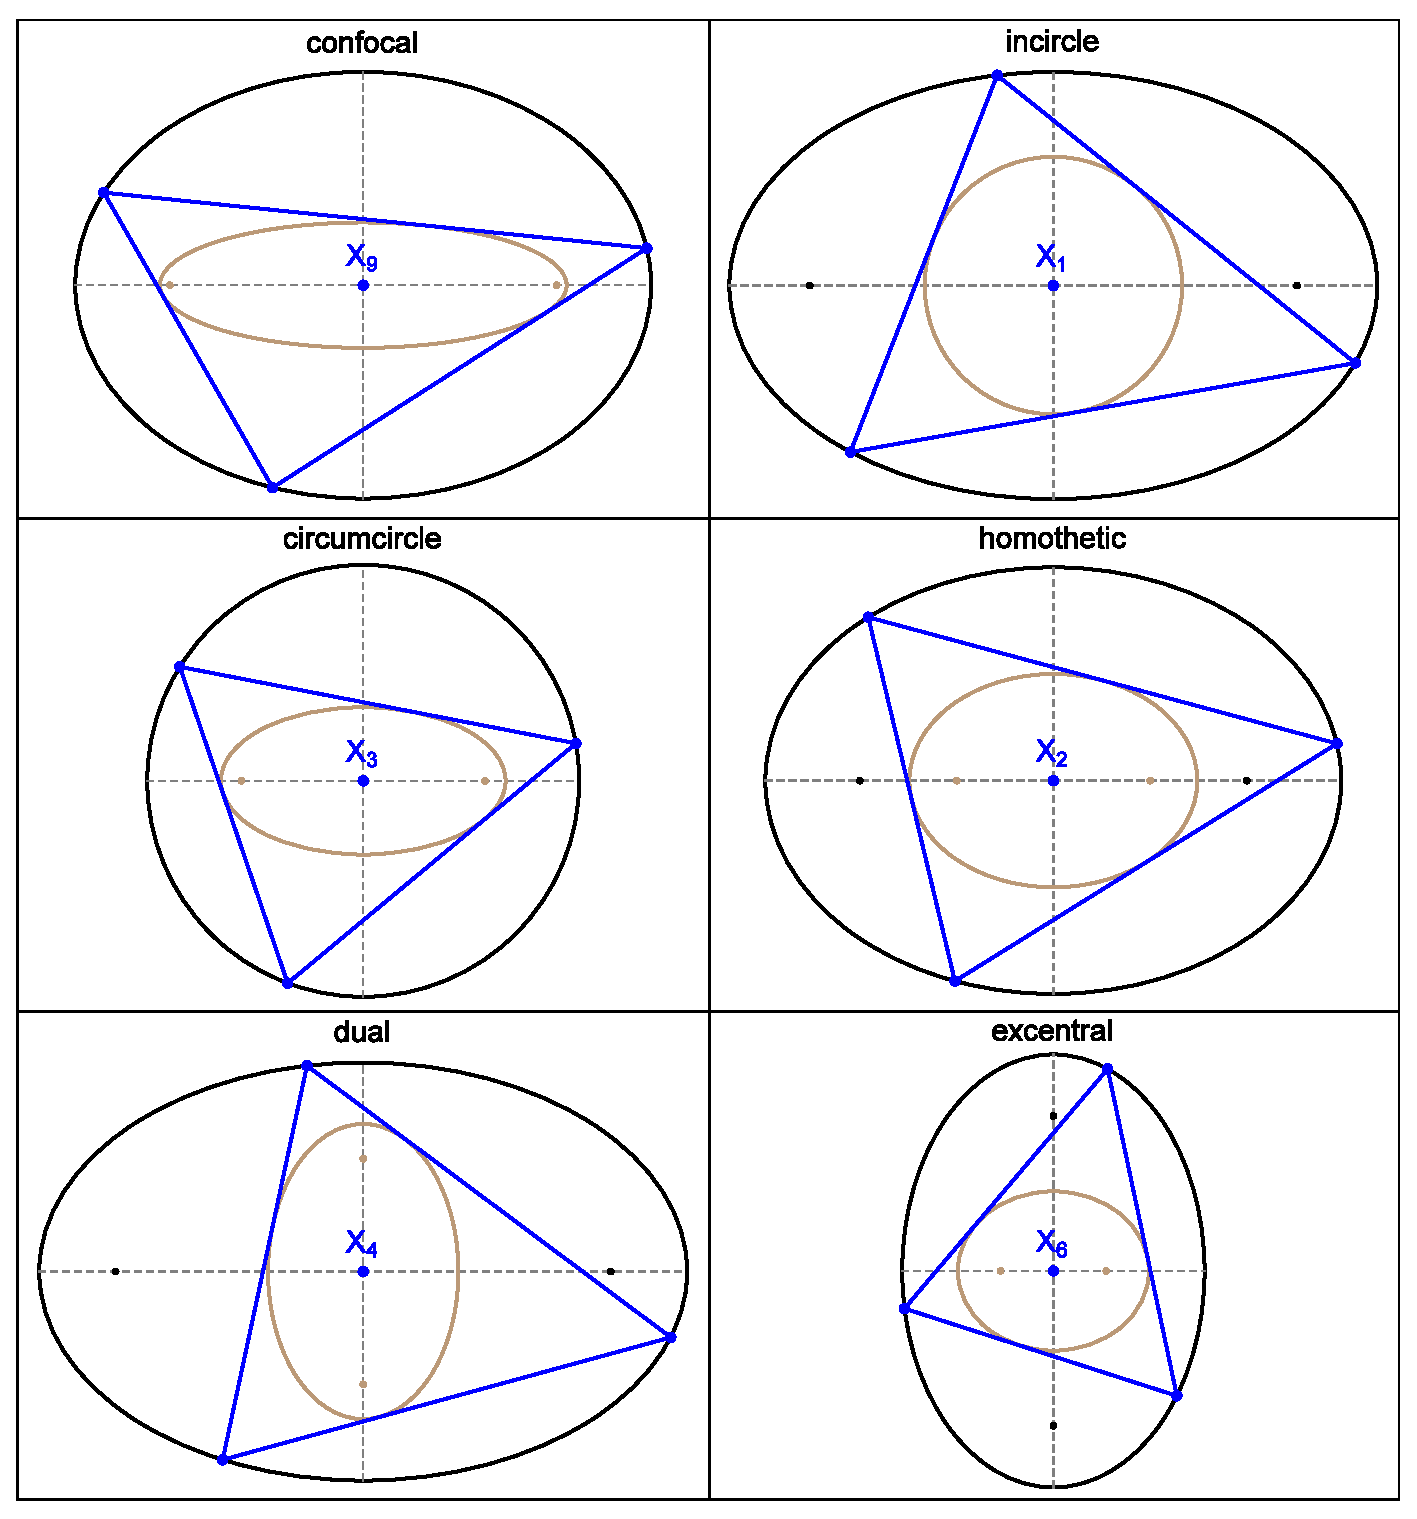
\includegraphics[width=\textwidth]{chap_06/pics/pics_06_015_six_caps_perp}
    \caption{The five concentric, axis-parallel (CAP) families whose loci are studied in this chapter. The confocal family is treated in \cref{chap:05-confocal-loci}. \href{https://youtu.be/14TQ5WlZxUw}{Video}}
    \label{fig:06-six-caps}
\end{figure}

Recall Cayley's condition for a CAP pair to admit a Poncelet 3-periodic family: $a_c/a+b_c/b=1$, where $a>b>0$, $a_c>0$, and $b_c>0$.




\section{Review: Jacobi's parametrization for bicentric polygons}
\label{sec:06-jacobi}
\input{chap_06/06_030_jacobi}

\section{Bicentric Family: Invariant Sum of Cosines}
\label{sec:06-bicentric-sum-of-cosines}


\begin{theorem}
The sum of cosines of angles internal to the family of N-periodics interscribed in a bicentric pair is invariant.
\label{thm:bicentric-sum}
\end{theorem}

\begin{proof}
Let $\{p_{j}(u)\}$, as in  \eqref{jacobivertex}, denote the vertices of the family of bicentric polygons. Let $\theta_{j}(u)$ denote the internal angle at the vertex $p_{j}(u)$. It follows from elementary geometry that
$\cos{\theta_{j}(u)}=-\cos({\phi_{j+1}(u)-\phi_{j-1}(u)}).$
Thus, if we denote by $S(u)$ the sum of the cosines of the internal angles, we have:

\begin{equation}
\label{sumofcosines}
S(u)=\sum \cos{\theta_{j}(u)}=-\sum{cn(u_{j+1})cn(u_{j-1})+sn(u_{j+1})cn(u_{j-1})},
\end{equation}
where $u_{j}=u+j\sigma$.

We now consider the natural complexified version of $S(u)$ defined on the complex plane by assuming that $u$ is a complex variable. To prove that $S$ is constant, it is sufficient to show that it has no poles and then apply Liouville's theorem.

So, suppose that $u=u_p$ is a pole of $S$. This implies that, for a certain index $j$, $u_{j}=u_{p}+j\sigma$ is a common pole of $cn(z)$ and $sn(z)$. We will now see that this leads to a contradiction.

In fact, by looking at (\ref{sumofcosines}), the terms where $u_{j}$ appears are given by
$$-(cn(u_{j})cn(u_{j-2})-sn(u_{j})cn(u_{j-2})+cn(u_{j+2})cn(u_{j})-sn(u_{j+2})cn(u_{j})).$$

Thus, the coefficients of $cn(u_{j})$ and $sn(u_{j})$ are, respectively:

$$-(cn(u_{j-2})+cn(u_{j+2})),$$

$$-(sn(u_{j-2})+sn(u_{j+2})).$$

Note that by (\ref{eqn:zpole}) both coefficients are zero, and they cancel out the simple poles of $cn(z)$ and $sn(z)$ at $u_{j}$, so $u_{p}$ is not a pole of $S$.   
\end{proof}

  

 %\section{Bicentric Limiting Pedals: Invariant Perimeter}
%\label{sec:pedal-perimeter}
%\input{chap_05/05_050_bicentric}  

\section{Bicentric Limiting Pedals: Invariant Perimeter}
\label{sec:06-pedal-perimeter}
\input{chap_06/06_060_pedal_perimeter}  

\section{A Tale of Five Polygons}
\label{sec:06-five-polys}
\input{chap_06/06_070_five_polys}  

%\section{List of Videos}
%\label{sec:videos}
%\input{090_videos}

 
\section{Polar Pedal Transformations}
\label{sec:06-polar-pedal}
\input{chap_06/06_220_app_bicentric_to_confocal} 
\section{Limiting Pedal Perimeters}
\label{sec:06-explicit-perimeter}
Using the identities

\begin{align*}
    sn(u+v)&={\frac {sn \left( u \right) cn \left( v \right) dn
 \left( v \right) +sn \left( v \right) cn \left( u
 \right) dn \left( u \right) }{\Delta \left( u,v \right) }}
\\
cn(u+v)&={\frac {cn \left( u \right) cn \left( v \right) -sn
 \left( u \right) sn \left( v \right) dn \left( u \right) 
dn \left( v \right) }{\Delta \left( u,v \right) }}
\\
dn(u+v)&={\frac {dn \left( u \right) dn \left( v \right) -{k}^{2}{
\it sn} \left( u \right) sn \left( v \right) cn \left( u
 \right) cn \left( v \right) }{\Delta \left( u,v \right) }}\\
\Delta(u,v)&=1-k^2 sn^2u\, sn^2v,\;\;\;  dn^2(u)+k^2sn^2(u)=1
\end{align*}
It follows that 

\[L_\pm(u)=L_\pm(0)=2 \,cn(\sigma)
sn(\sigma) \frac{\sqrt{ \delta_{\pm}R}}{k} \sum_{j=1}^{N}
  \,\frac{
  dn^2(j \sigma) }{  1-   \left(1-  dn^{2}(j \sigma) \right) 
  sn^{2}(\sigma)}
\]

\noindent where as before $\sigma=(4 \tau K)/N$.








\section{Bicentric Vertices:\torp{$N$}{N} = 3, 4}
\label{sec:06=bicentric-vertices-n34}
Consider a pair of circles
\[\mathcal{C}_1: x^2+y^2-r^2=0, \;\;\; \mathcal{C}_2: (x+d)^2+y^2-R^2=0\]

\subsection{N=3}

Let $(x_0,y_0)=(r\cos t,r\sin t) \in \mathcal{C}_1$. Let
$d^2=R(R-2r)$. Then the 3-periodic orbit is parametrized by
$\{P_1,P_2,P_3 \}, $ where
{\small  
\begin{align*}
P_1&=\left[{\frac {\cos t(2\,d R    \cos  t    +    {R}^{2}-  {d}^{2})+\Delta\,\sin t}{2\,R}}-d, {\frac {\sin t( 2d R\, \cos
 t  +  {R}^{2}-d^2) -\Delta\,\cos t }{2\,R}}\right]
\\
P_2&=\left[ {\frac { \cos t(2\,d R  \cos t     +{R}^{2}- {d}^{2})-\Delta\,\sin
 t }{2\,R}}-d,{\frac {\sin t(2d R\,  \cos
 t  +   {R}^{2}-  {d}^{2})+\Delta\,\cos t }{2\,R}}\right]
\\
 P_3&=\left[-{\frac { \left( R\cos t   -d \right)  \left( {R}^{2}-{d
}^{2} \right) }{     R^2+d^2-2\,d R\cos t }   }, {\frac 
{ -R\left(   R^2-d^2 \right) \sin t }{ R^2+d^2-2\,d R \cos
 t  }}\right]\\
 \Delta&=\sqrt { \left(  R^2+d^2-2d R\,\cos t   \right) 
 \left(   3\, R^2-d^2 +2\,d R\cos t\right) }
 \end{align*}
 }
Under the above pair of circles, the limiting points are at:

\begin{align*}
    l_1&=\left[\frac{  R^2-d^2 }{8\,d {R}^{2} }
 \left( \sqrt {   (9\,R^2-d^2)    
  (R^2-d^2)     }+3\, R^2+d^2 \right) 
,0\right]\\
l_2&=l_1-\left[\frac{\sqrt{9R^2 - d^2} (R^2-d^2)^{\frac{3}{2}}}{4R^2d}, 0\right].
\end{align*}
 
\subsection{N=4}

Let $(x_0,y_0)\in \mathcal{C}_1$. 
The Cayley condition for a pair of circles to admit Poncelet 4-periodics due to Kerawala is \cite[Poncelet's Porism, Eq. 39]{mw}:

\[ \frac{1}{(R-d)^2}+ \frac{1}{(R+d)^2}-\frac{1}{r^2}=0 \]
  
Let $P_i=[x_i,y_i]$, $i=1,...,4$ denote the vertices of a bicentric 4-periodic. Let $\alpha=R^2+d^2$ and $\beta=R^2-d^2$. The vertices are parametrized as:
 
\begin{align*}
\small
   x_{1}&=\Delta\,y_0-{\frac { \left( \beta+2\,d x_0
 \right)  \left( d \alpha  -\beta x_0 \right) }{2\,\alpha}},\\
 y_{1}&=-\Delta\,x_0+{\frac { \left( 2\,d \beta x_0+
 \alpha ^{2} \right) y_0}{2\,\alpha}}\\
x_{2}&=-\Delta\,y_0-{\frac { \left( \beta+2\,dx_0
 \right)  \left( d \beta - \beta x_0 \right) }{2\,\alpha}}\\
y_{2}&=\Delta\,x_0+{\frac {2\,d \beta y_0\,x_0+
 \alpha ^{2}y_0}{2\,\alpha}}\\
%
 x_3&= \frac{  ((( x_0^2 \alpha \beta - 4  x_0^2 \alpha^2 + 3/2 \beta^3 - 2 \beta^2 \alpha) \sqrt{2 \alpha - 2 \beta} + \beta (2 \Delta \alpha  y_0 + 8 \alpha^2  x_0 - 8 \alpha \beta  x_0 + \beta^2  x_0)) \beta)}{(4 (\sqrt{2 \alpha - 2 \beta} \alpha  x_0 + \beta (\beta - 2 \alpha)/2)^2)}\\
 y_3&=\frac{\alpha \beta (\alpha (2  x_0  y_0 \alpha + \beta ( x_0  y_0 - 2 \Delta)) \sqrt{2 \alpha - 2 \beta} + (4 \Delta  x_0 - 2 \beta  y_0) \alpha^2 - 2 \Delta \alpha \beta  x_0 + \beta^3  y_0)}{(2 \sqrt{2 \alpha - 2 \beta} \alpha  x_0 - 2 \alpha \beta + \beta^2)^2}\\
 x_4&=-\frac{((( x_0^2 \alpha \beta - 4  x_0^2 \alpha^2 + 3/2 \beta^3 - 2 \beta^2 \alpha) \sqrt{2 \alpha - 2 \beta} + \beta (-2 \Delta \alpha  y_0 + 8 \alpha^2  x_0 - 8 \alpha \beta  x_0 + \beta^2  x_0)) \beta)}{(4 (\sqrt{2 \alpha - 2 \beta} \alpha  x_0 + \beta (\beta - 2 \alpha)/2)^2)}\\
 y_4&=\frac{(\alpha (2  x_0  y_0 \alpha + \beta ( x_0  y_0 + 2 \Delta)) \sqrt{2 \alpha - 2 \beta} + (-4 \Delta  x_0 - 2 \beta  y_0) \alpha^2 + 2 \Delta \alpha \beta  x_0 + \beta^3  y_0) \beta}{(2 \sqrt{2 \alpha - 2 \beta} \alpha  x_0 - 2 \alpha \beta + \beta^2)^2}\\
 \Delta&=\frac{\sqrt{-2\sqrt{2\alpha - 2\beta}\; \alpha x_0\beta^2 - 2 x_0^2\alpha^3 + 2 x_0^2\alpha^2\beta + \alpha^2\beta^2 + \alpha\beta^3 - \beta^4}}{ (2\alpha}
\end{align*}

Under the above pair of circles, the limiting points are at:
\begin{align*}
    l_1=\left[\frac{R^2 - d^2}{2d}, 0\right],\;\;\; l_2=  \left[\frac{d(R^2-d^2)}{R^2 + d^2}, 0\right]
\end{align*} 

\section{Limiting Pedal Perimeters for \torp{$N$}{N} =3 and \torp{$N$}{N} =4}
\label{sec:06-pedal-perimeters-n34}
 \input{chap_06/06_260_app_pedal_perimeters_n34}
 

\section{Exercises}
\label{sec:06-exercises}
\section{Exercises}

\begin{exercise}
Prove that over incircle 3-periodics, the power of the center with respect to the (fixed radius) circumcircle is invariant and  equal to $-a b$.
\end{exercise}

\begin{exercise}
Compute $a/b$ of the external ellipse in the incircle CAP family such that (i) the circular locus of $X_3$ coincides with the incircle, (ii) the elliptic locus of $X_4$ touches the outer ellipse at its top and bottom vertices, and (iii) the circular locus of $X_5$ coincides with the incircle. See it \href{https://bit.ly/3wzw1CD}{Live1}, \href{https://bit.ly/3vnVHlL}{Live2}.
\end{exercise}

\begin{exercise}
Derive the radius of the circumcircle in the same-named family such that the quartic locus of $X_1$ and the circular locus of $X_4$ intersect at four points on the inner ellipse, see it \href{https://bit.ly/3wzQkjp}{Live}. 
\end{exercise}

\begin{exercise}
Prove \cref{prop:06-homoth-four-circles}.
\end{exercise}

\begin{exercise}
Prove that over homothetic 3-periodics, the radius of the circular locus of $X_{16}$ is minimum when $a/b=3$.
\end{exercise}

\begin{exercise}
Prove that at $a/b=\sqrt{5}$, the elliptic loci of the Brocard points over homothetic 3-periodics are internally tangent to the inner ellipse.  See it \href{https://bit.ly/3fkEMuG}{Live}.
\end{exercise}

\begin{exercise}
Derive the $a/b$ such that the elliptic loci of the Brocard points over the homothetic family intersect the y axis at $b/2$, i.e., at the top vertex of the caustic. See it \href{https://bit.ly/3fm8G1u}{Live}.
\end{exercise}

\begin{exercise}
Prove that over homothetic 3-periodics, the locus of the Brocard midpoint $X_{39}$ is an ellipse, derive its axis.
\end{exercise}

\begin{exercise}
Show that over homothetic 3-periodics, the elliptic locus of the vertices of the first Brocard triangle is interior to the inner ellipse.
\end{exercise}

\begin{exercise}
Compute the invariant similarity ratio of homothetic 3-periodics to the first Brocard triangles. 
\end{exercise}

\begin{exercise}
Derive expressions for the areas in \cref{cor:06-equi-areas}.
\end{exercise}

\begin{exercise}
Synthesize a triangle center such that over billiard 3-periodics its locus is a circle? Hint: it will be an affine combination of $X_2$ and $X_3$.
\end{exercise}

\begin{exercise}
Derive semi-axes for the dual family elliptic loci of $X_2$, $X_3$, and $X_5$ in \cref{prop:06-dual-x2345}.
\end{exercise}

\begin{exercise}
As shown in \cref{sec:06-ncap-loci}, over poristic triangles, the locus of $X_{44}$, and $X_{171}$ are segments. Derive their data. Do the same for the segment-loci of $X_{50}$, $X_{52}$, $X_{58}$ over Brocard porism 3-periodics.
\end{exercise}

\begin{exercise}
Given an ellipse $\E$ with semi-axes $a$, $b$, consider a non-Ponceletian family of triangles with two vertices fixed on the foci of $\E$ and a third one which sweeps the boundary. Show the locus of the incenter of this family is an ellipse. See it \href{https://bit.ly/3up4a6V}{Live}.
\end{exercise}

\begin{exercise}
Prove that over the Brocard porism, the locus of $X_{114}$ is a circle concentric with, and exterior to, the Brocard inellipse. Derive its radius. \href{https://bit.ly/3g6pmcv}{Live}
\end{exercise}

\begin{exercise}
Prove that over the Brocard porism, the locus of $X_{115}$ is a circle concentric with the Brocard inellipse of radius equal to the latter's minor semi-axis. \href{https://bit.ly/3pfR5Mc}{Live}
\end{exercise}

\begin{exercise}
Over the Brocard porism, the locus of $X_{185}$ is an ellipse which intersects the major axis of the Brocard inellipse $\E'$ in two points $A$ and $B$, see it \href{https://bit.ly/2Rn0chC}{Live}. In the $1<a/b<2$ range, $A,B$ appear to lie between the foci of $\E'$, however for larger $a/b$, e.g., $a/b=3$, the locus seems to pass through the foci, see it \href{https://bit.ly/3icu7Eh}{Live}. Prove or disprove this statement. Derive the center and semi-axes of the locus. 
\end{exercise}
